\documentclass[a4paper, 11pt]{article}
\usepackage[left=0.9in,right=0.9in,bottom=0.9in,top=0.9in]{geometry}
\usepackage{amsmath}
\usepackage{multicol}
\usepackage{graphicx}
\setlength{\columnsep}{0.7cm}
\usepackage{tabto}
\usepackage{lipsum}
\usepackage[small]{titlesec}
\usepackage[]{natbib}
\bibliographystyle{plainnat}
\setcitestyle{authoryear, open={((},close={)}}
\usepackage{hyperref}
\hypersetup{colorlinks=false}
\setlength{\bibsep}{0pt plus 0.3ex}
\usepackage[none]{hyphenat}
\usepackage{float}
\usepackage{multirow}
\usepackage[T1,hyphens]{url}
\setlength\parskip{0pt}
\let\olditemize=\itemize \let\endolditemize=\enditemize \renewenvironment{itemize}{\olditemize \itemsep-0.33em}{\endolditemize} 
\usepackage{caption}
\usepackage{subcaption}
\usepackage{rotating}

%for code
\usepackage{listings}
\usepackage{color}

\definecolor{dkgreen}{rgb}{0,0.6,0}
\definecolor{gray}{rgb}{0.5,0.5,0.5}
\definecolor{mauve}{rgb}{0.58,0,0.82}

\lstset{frame=tb,
  language=Python,
  aboveskip=3mm,
  belowskip=3mm,
  showstringspaces=false,
  columns=flexible,
  basicstyle={\small\ttfamily},
  numbers=none,
  numberstyle=\tiny\color{gray},
  keywordstyle=\color{blue},
  commentstyle=\color{dkgreen},
  stringstyle=\color{mauve},
  breaklines=true,
  breakatwhitespace=true,
  tabsize=2
}

\title{\vspace{-25mm} Machine Learning Methods for Classification of Deceptful Reviews}
\author{ Dimitar Angelov (2339463)\\Yuxuan Hou (4962273)\\Angel Temelko (8221113)\\\\ Practical Assignment 2, Data Mining\\ Utrecht University \vspace{-3.6mm}}
\date{05.11.2021}

\begin{document}
	\maketitle
	\vspace{-6mm}
	
	\begin{abstract}
		\noindent
		Due to the presence of malicious comments on the web, we have used techniques such as machine learning for text classification based on the theory and data already available from Ott et al. to try to discern false comments hidden in real comments. By training the model, we obtained a classification result with a maximum value of 89.99\% for F1. We also compared the use of Uni-grams, Bi-grams, and both Uni-grams and Bi-grams. The five most important feature values pointing to false and true reviews were found and analyzed.
	\end{abstract}

\begin{multicols}{2}
\maketitle

\section{Introduction}

% With the development of the internet, people can easily go to some booking sites to arrange their travel plans, such as what kind of hotels to stay in, etc. Then when booking, some of the reviews under this hotel will largely influence the guest's choice of this hotel. After all, it stands to reason that if people see that the hotel is dirty and noisy, then they will not choose it. Businessmen find out about this and hire people to maliciously post negative reviews about their competing hotels. Such false reviews are hidden in the real reviews and are difficult for travellers to uncover, thus causing the hotel to lose money. 

With the growth of the internet, online booking and shopping has become mainstream. Reviews of an item will largely influence people's perception of that item. Take Amazon.com, for example, as one of the largest e-commerce sites, reviews are very important to them. This is because their business model is to gain the trust of their users so that they can quickly place an order for an item. In this case, it becomes easy to have malicious bad reviews. That is, there are false negative reviews that are difficult to distinguish in order to disrupt the user's choice. To distinguish fake reviews from multiple reviews, many researchers are currently trying to solve them using knowledge such as machine learning.

Many researchers are currently attempting to address it using knowledge from multiple perspectives. For example, \cite{1} use PU-learning in their report, building a binary classifier based on positive, to discriminate negative deceptive opinion spams. Not only that, but \cite{2} also mention the use of natural language processing to extract meaningful features from the text, as well as the use of machine learning techniques to devise methods for further investigation. In \cite{3}, the authors design a system with the innovative use of (i) sentiments of review and its comments, (ii) content-based factor, and (iii) rating deviation, to implement a stand-alone system that can be used to filter product review datasets.

We will use a total of 800 fake and genuine hotel reviews, presented in \cite{ott2011finding, ott2013negative} Based on the theoretical basis shown in \cite{ott2011finding, ott2013negative} for examining the weights of features learned by machine learning classifiers, we use machine learning to train the data and classify deceptive, false reviews based on similar text, and use Multinomial Naive Bayes to generate a linear classifier, and Logistic Regression to classifier to discriminate, and use classification trees and random forests for flexible classification. This paper will clearly describe the analysis process, measure the results using metrics such as precision, recall, F1 scores, and analyze and collate the results.

\section{Data Description}

The data for this project was obtained from  \href{https://myleott.com/op-spam.html}{myleott.com}, \cite{ott2011finding, ott2013negative}. It contains hotel reviews for 20 Chicago hotels, and there are four categories: truthful positive, deceptive positive, truthful negative, deceptive negative. Each of the categories contains 400 reviews.

Within these reviews, we will focus on deceptive opinion spam. Below we give some examples of sentences from deceptive negative reviews and true negative reviews:
\begin{quote}
{\emph {\footnotesize1. When I got home, I washed all my clothes whether I had worn them or not, such was the skeeviness of our accomodations. Please, do yourself a favor and stay at a CLEAN hotel. [deceptive]}}
\end{quote}
\begin{quote}
{\emph {\footnotesize2. My \$200 Gucci sunglasses were stolen out of my bag on the 16th. I filed a report with the hotel security and am anxious to hear back from them. This was such a disappointment, as we liked the hotel and were having a great time in Chicago. [truthful]}}
\end{quote}

To obtain truly deceptive reviews, \cite{ott2011finding, ott2013negative} collected data form Mechanical Turk. Workers wrote these deceptive negative reviews from the point of view of a person at one of Chicago's most famous hotels, who would imagine and write a false negative review about a rival hotel. Each review was high quality, had the correct hotel information, was readable and not plagiarised, and conveyed a negative sentiment. The average length of these negative fake reviews was also higher than that of the positive reviews.

The real reviews were from Expedia, Hotels.com, Orbitz, Priceline, TripAdvisor, and Yelp. \cite{ott2011finding, ott2013negative} show that the deception rate for these review sites is relatively low. We will take a subset of the existing real reviews and use them to compare the deceptive reviews.

\section{Methods}

The data was pre-split into five folds. We used four folds in the sample for model training and parameter tuning and fold 5 for estimating the performance of the classifiers.

For the project, we used the scikit-learn (\cite{scikit-learn}) implementations of the statistical measures Multinomial Naïve Bayes, Logistic Regression, Classification Trees, Random Forests, and NLTK library (\cite{journals/corr/cs-CL-0205028, bird2009natural}) to get a list of stop words, as well as implementations of methods for stemming and lemmatization.

\subsection{Pre-processing}
Firstly, we read each review from the text files in the data and create a separate corresponding list of their labels. Since the data was already split into folds that we use as a separator for the training and testing set, we did not need to perform a train/test split. 

The text was then split into a vector of Uni-grams, Bi-grams, or a combination of Uni-grams and Bi-grams, using the \emph{CountVectorizer} method from scikit-learn. This is a standard method in NLP. We are using Uni-grams and Bi-grams to learn the program about the patterns of the words, and combining both of them will produce better results but more complex.

There are several methods to perform word normalization and text pre-processing. We wanted to test several different ones to examine the effect different techniques will have on the performance of the classifiers. In addition to the three configurations of n-grams, we also tested combinations of 4 pre-processing parameters. Both the training and the test data was pre-processed in an identical configuration.

\subsubsection{Lowercasing}

We are making all of the words lowercase. This step was always performed in our research. It is essentially the most basic type of pre-processing. Since the text is transformed into a BOW representation of n-grams, having uppercase characters will add little to no information at the expense of a more significant number of n-grams.

\subsubsection{Removing Stop Words}
Stop words are any list of words that are removed from the data. Usually, these are prevalent words that have been found to add no information to the meaning of a sentence. There is no agreed-upon list of universally used words, and they can vary significantly in size. The list we chose is the English list of stop words in the NLTK package, which contains 127 words. You can see it in the appendix \ref{appendix:words}. 

\subsubsection{Stemming}
Stemming maps different forms of the same word to a common "stem" - for example, the words \emph{connection}, \emph{connections}, \emph{connective}, \emph{connected}, and \emph{connecting} would all be converted to \emph{connect}. As with all natural language pre-processing, there is a trade-off between information and noise when using this method. There are different stemming algorithms, and there is not one universally agreed upon as the best. We chose to use the NLTK implementation of the \emph{snowball} (also known as Porter2) algorithm. \cite{porter1980algorithm}.

\subsubsection{Lemmatization}
Lemmatization has a similar goal to stemming - to reduce a word into its base form. Implementations will generally use more sophisticated methods to get to their results. Much like stemming, there are many different algorithms and methods to perform lemmatization. For our project, we used the NLTK implementation of the \emph{WordNet} corpus' lemmatizer.\cite{porter1980algorithm}

\end{multicols}
\subsubsection{Pre-processing Implementation}

\begin{lstlisting}
from data_in import df_training, df_testing
from nltk.stem import SnowballStemmer
from nltk.stem import WordNetLemmatizer
import re

from config import ngram_range, min_df
from config import lowercase, remove_stops, stemming, lemmatization

# adapted from https://www.kaggle.com/anu0012/basic-approach-with-neural-network
def cleanData(text, lowercase, remove_stops, stemming, lemmatization):
    txt = str(text)

    txt = re.sub(r'[^A-Za-z\s]', r' ', txt)

    if lowercase:
        txt = " ".join([w.lower() for w in txt.split()])

    if remove_stops:
        txt = " ".join([w for w in txt.split() if w not in stops])

    if stemming:
        st = SnowballStemmer(language='english')
        txt = " ".join([st.stem(w) for w in txt.split()])

    if lemmatization:
        wordnet_lemmatizer = WordNetLemmatizer()
        txt = " ".join([wordnet_lemmatizer.lemmatize(w, pos='v') for w in txt.split()])

    return txt

# clean text
X_train = X_train.map(lambda x: cleanData(x, lowercase=lowercase, 
    remove_stops=remove_stops, stemming=stemming, lemmatization=lemmatization))
X_test = X_test.map(lambda x: cleanData(x, lowercase=lowercase, 
    remove_stops=remove_stops, stemming=stemming, lemmatization=lemmatization))

\end{lstlisting}

\begin{multicols}{2}

\subsection{Models}

After performing text normalization on both the training and testing test, we trained classifiers using the following 4 classification techniques:
\begin{itemize}
    \item Multinomial Naïve Bayes
    \item Logistic Regression
    \item Classification Trees
    \item Random Forests
\end{itemize}

For each of the above, the respective implementation in the scikit-learn library \cite{scikit-learn} was used. 

\subsubsection{Multinomial Naïve Bayes}
Naïve Bayes (NB) classifiers are some of the most computationally simple classifiers commonly used for Machine Learning. Despite their relative simplicity and low data requirements, naïve bayes classifiers have been demonstrated to work well in many real-world applications, especially in NLP, such as document classification and spam filtering. (\cite{Mccallum1998, Metsis2006}).

\subsubsection{Logistic Regression}
The Logistic Regression is a classification algorithm used to analyze the connection between the dependent variable and one or more independent variables. It is mainly used to work with binary data, predicting two values (true or false). It was introduced by \cite{peng2002introduction}. The real-world application of logistic regression would be predicting something that has two values, like predicting if the mail is spam or not spam, and in this case, if the review is fake or genuine. It works well when the data can be separated linearly. The disadvantage of this classification algorithm is bad for predicting continuous and discrete data. The advantage is that it is easier to implement than other methods.

\subsubsection{Decision Trees}
The decision tree (DT) classifier (or classification tree) continuously splits the data according to a set of features. It begins with a ‘root’ node and has several branches (features) and leaves (labels). Data is split along branches to maximize information gained per split (different measures of information gained can be used). The data continues to be split until the first of several scenarios occurs: a pre-specified maximum depth is reached; a branch has all the same values of leaves, or when splitting no longer adds value to the predictions (\cite{morgan1963problems}).

Decision trees are relatively simple to understand and interpret due to the boolean logic used to make decisions. They are computationally quick and straightforward to both train and infer. One of the main hurdles for decision trees is that they are prone to overfit the training set. There are several ways to minimize this, the most common and straightforward is setting a maximum number of splits (depth).

\subsubsection{Random Forests}
The random forest (RF) algorithm is an ensemble learning model – it uses the output of several other models in order to make predictions (\cite{ho1995random}). RFs use many shallow decision tree models, each of which is trained on a bootstrap-sampled subset of the training set. Furthermore, when deciding the split for each branch during the training of the trees, the best split is found from a random subset of size
\(max\_features\). Generally, on inference, each decision tree will predict the input, and the class that was picked the highest number of times will be chosen as the output.

Note that the sci-kit learn implementation differs from this and the output will be taken by “averaging their probabilistic prediction, instead of letting each classifier vote for a single class”.\footnote{\href{https://scikit-learn.org/stable/modules/generated/sklearn.ensemble.RandomForestClassifier.html}{Sci-Kit Learn Random Forest Implementation}\label{sklearn:rf}} This was initially proposed in \citet{Breiman1996}.

There are several advantages to random forests. They correct for decision trees' tendencies to overfitting to their training set and will generally outperform large individual decision trees. They are, however, generally considered to be black-box models, as there is no clear path taken to produce an output. As such, they can be more difficult to fine tune accurately and understand in general.


\subsubsection{Grid Search}
All models were trained using Grid Search with test accuracy used as the optimization function and 10-fold cross-validation. The following configurations for pre-processing were used:

\begin{itemize}\raggedright 
    \item Lowercasing
    \item Lowercasing, Stop words removed
    \item Lowercasing, Stop words removed, Stemming
    \item Lowercasing, Stop words removed, Lemmatization
\end{itemize}

The four configurations were tested on the data vectorized into Uni-grams, Bi-grams, and both Uni-grams and Bi-grams.

The hyper-parameters, shown in Table \ref{table:hyperparam}, were tuned for each dataset. You can see the hyper-parameters, F1-Score, and training time of all of the models on each of the datasets in section \ref{apx:results} of the appendix. The training time reported is the time it took to train the model with those specific hyperparameters and does not include the time taken to perform Grid Search over the total number of hyperparameters. All training and evaluation were done on an 8 thread Intel i7-4790 CPU.

\subsubsection{Statistical Analysis}
A McNemar test (\cite{mcnemar1947note}) was applied on the confusion matrices of the models with the highest classification accuracy on the test set. The McNemar test allows us to determine whether the number of false predictions for both positive and negative classes is equal for paired samples. It uses the Chi-Square distribution to determine the probability of difference.

If the $\chi^{2}$ result is significant, this provides sufficient evidence to reject the null hypothesis, in favor of the alternative hypothesis, that the number of false predictions for both positive and negative classes is significantly different from each other. We used a significance value of 0.05 for our tests.

\begin{equation}
     \chi ^{2}={\frac{(FP-FN)^{2}}{FP+FN}}
\end{equation}

In addition, we performed a 5x2cv paired t test, as proposed in \cite{dietterich1998approximate}, to evaluate if there is a statistically significant difference in the accuracy of pairs of classifiers. We used the implementation within the \emph{paired\_ttest\_5x2cv} method of the mlxtend package (\cite{raschkas_2018_mlxtend}).

\end{multicols}
\begin {table}[h]
\centering
\caption {All hyper-parameters which were tested for each model}
\begin{tabular}{l*{6}{c}r}
%\caption {All hyper-parameters which were tested for each model}
\hline
Algorithm                         &  Hyper parameters tested \\
\hline
\hline
Multionmial Naive Bayes          &  $Alpha: 0.01, 0.1, 0.25, 0.5, 1, 2.5, 10$ \\
\hline
Linear regression                & \begin{tabular}[c]{@{}l@{}}$Penalty: L1, L2$\\ $C: 0.01, 0.1, 0.25, 0.5, 1, 2.5, 5, 10$\end{tabular}
  \\
\hline
Decision Tree                    & \begin{tabular}[c]{@{}l@{}}$Max depth: None, 2, 4, 8, 16$ \\ $Min samples per split: 2, 4, 8, 16$\end{tabular} \\
\hline
Random Forest                    & \begin{tabular}[c]{@{}l@{}}$N estimators: 10, 50, 100, 500, 1000$\\  $Max depth: None, 2, 4, 8, 16$ \\ $Min samples per split: 2, 4, 8, 16$\end{tabular} \\
\hline
\end{tabular}
\label{table:hyperparam}
\end{table}

\clearpage
\subsubsection{Classifier Implementation}
A summarized version of the code for the training, tuning, and testing procedure.
\begin{lstlisting}
from sklearn.model_selection import GridSearchCV

from sklearn.naive_bayes import MultinomialNB
from sklearn.linear_model import LogisticRegression
from sklearn.tree import DecisionTreeClassifier
from sklearn.ensemble import RandomForestClassifier

from data_preprocessing import train, y_train, test, y_test
from getResults import getResults

# --------------------------
# Naive Bayes
NB_paramGrid = {'alpha': [0.01, 0.1, 0.25, 0.5, 1, 2.5, 10]}

NB_gridSearch_model = GridSearchCV(MultinomialNB(), NB_paramGrid, cv=10, n_jobs=-1)
NB_gridSearch_model.fit(train, y_train)

y_pred = NB_gridSearch_model.predict(test)

# --------------------------
# Logistic Regression
LR_paramGrid = {'penalty': ['l1', 'l2'], 'C': [0.01, 0.1, 0.25, 0.5, 1, 2.5, 5, 10]}

LR_gridSearch_model = GridSearchCV(LogisticRegression(solver='liblinear'), 
    LR_paramGrid, cv=10, n_jobs=-1)
LR_gridSearch_model.fit(train, y_train)

y_pred = LR_gridSearch_model.predict(test)

# --------------------------
# Classification Trees
DT_paramGrid = {'max_depth': [None, 2, 4, 8, 16], 'min_samples_split': [2, 4, 8, 16]}

DT_gridSearch_model = GridSearchCV(DecisionTreeClassifier(), 
    DT_paramGrid, cv=10, n_jobs=-1)
DT_gridSearch_model.fit(train, y_train)

y_pred = DT_gridSearch_model.predict(test)

# --------------------------
# Random Forests
RF_paramGrid = {'n_estimators': [10, 50, 100, 500, 1000],
                'max_depth': [None, 2, 4, 8, 16], 'min_samples_split': [2, 4, 8, 16]}

RF_gridSearch_model = GridSearchCV(RandomForestClassifier(), 
    RF_paramGrid, cv=10, n_jobs=-1)
RF_gridSearch_model.fit(train, y_train)

y_pred = RF_gridSearch_model.predict(test)
\end{lstlisting}
\clearpage

\begin{multicols}{2}

\section{Results}

You can see a plot of the results in Fig. \ref{results:perf}. In the figure are presented the test metrics for the best performing model for each classification technique. In addition, we have tracked the training time for the models, which has been plotted in Fig. \ref{results:time}.

\subsection{Multinomial Naive Bayes}

The best performing Multinomial Naive Bayes classifier achieved an accuracy of 83.90\% on the test set and 96.25\% on the training set, with a precision of 0.868, recall of 0.868, and F1-Score of 0.868. The null-hypothesis of the McNemar test was not rejected (p=0.3458).

To achieve this result, Uni-grams were created on text data that was lowercased, stemmed, and had the stop words removed. For the hyper-parameters, \emph{Alpha=2.5} was found to give the best result.

The confusion matrix for the Multinomial Naive Bayes classifier can be seen in Fig. \ref{nb cm}.

\subsection{Logistic Regression}
The best performing Logistic Regression classifier achieved an accuracy of 86.71\% on the test set, with a precision of 0.846, recall of 0.843, and F1-Score of 0.843. The null-hypothesis of the McNemar test was not rejected (p=0.3173).

The data consisted of both Uni-grams and Bi-grams that were lowercased, stemmed, with the stop words removed. For the hyper-parameters, L2 regularization with a value for \emph{C=0.1} was found to give the best result.

The confusion matrix for the Logistic Regression classifier can be seen in Fig. \ref{lr cm}.

\subsection{Decision Tree}
The best performing Decision Tree classifier achieved an accuracy of 70.46\% on the test set and 73.90\% on the training set, with a precision of 0.643, recall of 0.643, and F1-Score of 0.643. The null-hypothesis of the McNemar test was not rejected (p=0.3538).

Uni-grams were created on text data that was lowercased, and had the stop words removed from it. It was not stemmed or lemamtized. For the hyper-parameters, (\emph{max\_depth=2}) and Minimum of 4 samples required in a leaf node to perform a split (\emph{min\_samples\_split=4}) were found to give the best result. 

The confusion matrix for the Decision Tree classifier can be seen in Fig. \ref{dt cm}.

\subsection{Random Forest}

The best performing Random Forest classifier achieved an accuracy of 85.62\% on the test set and 96.40\% on the training set, with a precision of 0.867, recall of 0.831, and F1-Score of 0.827. The null-hypothesis of the McNemar test was not rejected (p=0.0736). 

Both Uni-grams and Bi-grams were created on text data that was lowercased, stemmed, and had the stop words removed. For the hyper-parameters, a maximum depth of 4 (\emph{max\_depth=4}), minimum of 2 samples required in a leaf node to perform a split (\emph{min\_samples\_split=2}) and 1000 estimator trees (\emph{n\_estimators=1000}) was found to give the best result.

The confusion matrix for the Random Forest classifier is shown in Fig. \ref{rf cm}.


\subsection{Pre-processing}
With all of the results in mind, the best preprocessing configuration uses stemming, lowercases the text, and removes the stop words from it. It seems that lemmatization, or at least the implementation we used, was not able to perform well, as it consistently scored worse than when using stemming. You can see this in detail in Figure \ref{apx:results} in the appendix. In most cases, this configuration yielded the best results.

In most cases, using the combination of Uni-grams and Bi-grams produces the highest score, although it is not always the case. You can see a plot of the effect different n-grams had on the F1-score of each of the models in Fig. \ref{results:n-grams}. This is further explored in the Discussion section.

\end{multicols}
\begin{figure}
    \centering
    \begin{subfigure}[t]{0.7\textwidth}
        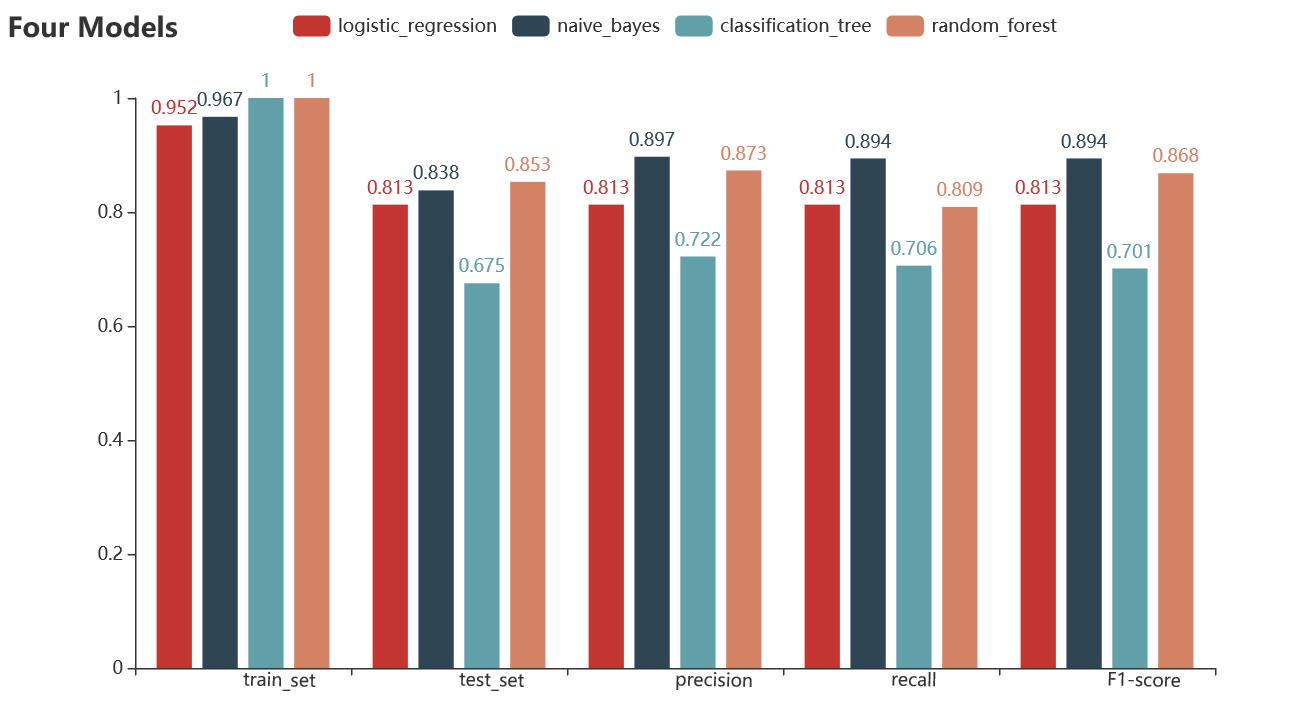
\includegraphics[width=\textwidth]{figures/four models(1).png}
        \caption{A comparison of several performance measures}\label{results:perf}
    \end{subfigure}
    \begin{subfigure}[t]{0.7\textwidth}
        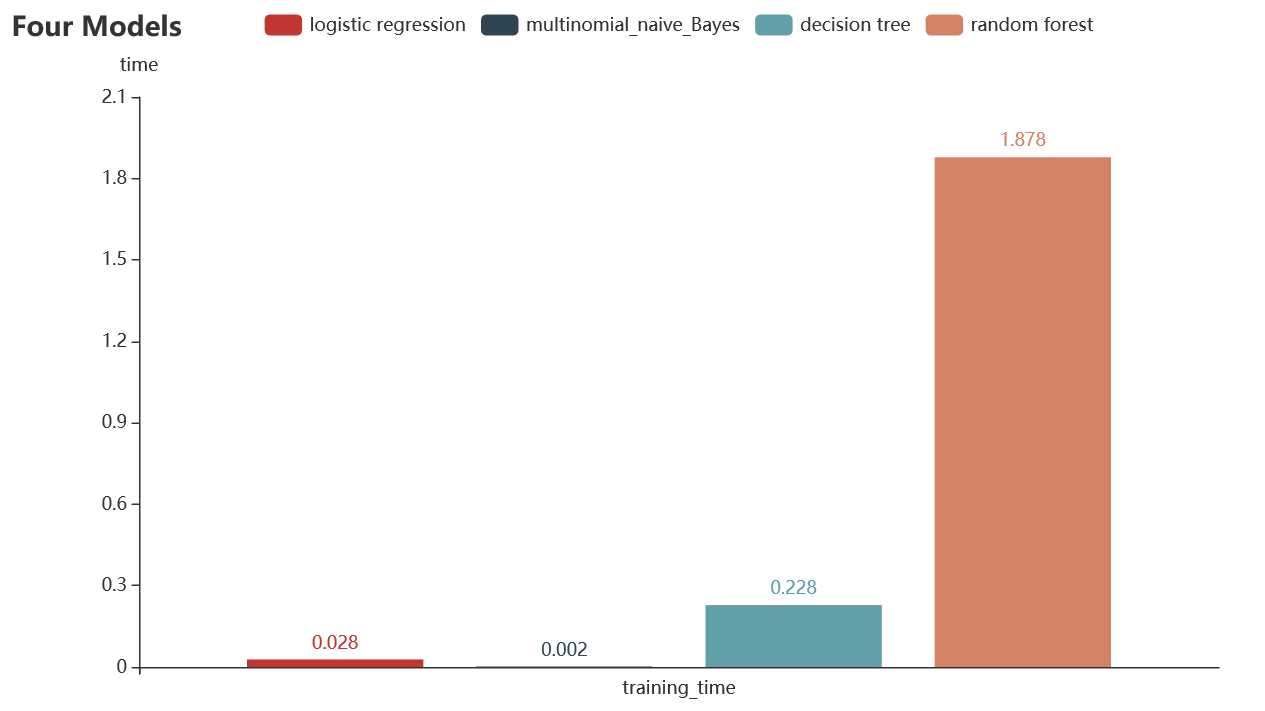
\includegraphics[width=\textwidth]{figures/training time.png}
        \caption{Training time of each model}\label{results:time}
    \end{subfigure}
    \begin{subfigure}[t]{0.7\textwidth}
        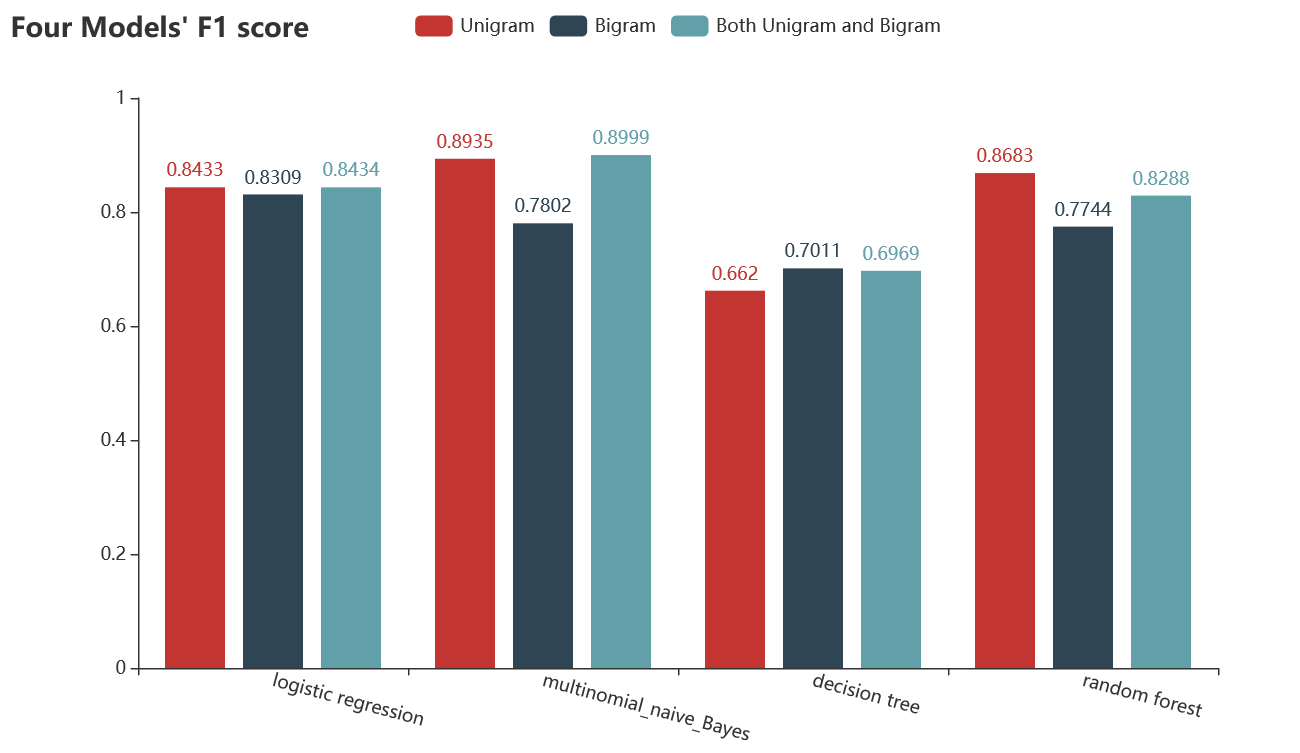
\includegraphics[width=\textwidth]{figures/Four Models' F1 score.png}
        \caption{Comparison of F1-score for the models depending on N-gram size}
        \label{results:n-grams}
    \end{subfigure}
\caption{}
\end{figure}

\begin{figure}
    \centering
    \begin{subfigure}[t]{0.45\textwidth}
        \centering
        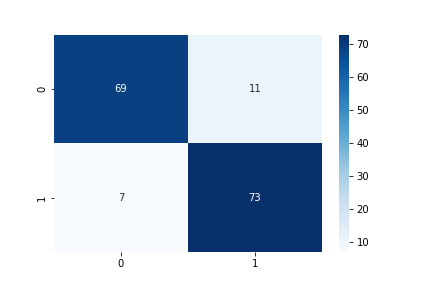
\includegraphics[width=\textwidth]{figures/MultinomialNB.png}
        \caption{Naive Bayes}\label{nb cm}
    \end{subfigure}
    \begin{subfigure}[t]{0.45\textwidth}
        \centering
        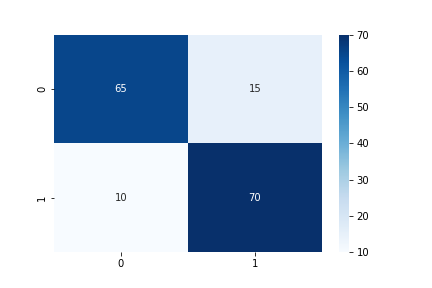
\includegraphics[width=\textwidth]{figures/LogisticRegression.png}
        \caption{Logistic Regression}\label{lr cm}
    \end{subfigure}
        \begin{subfigure}[t]{0.45\textwidth}
        \centering
        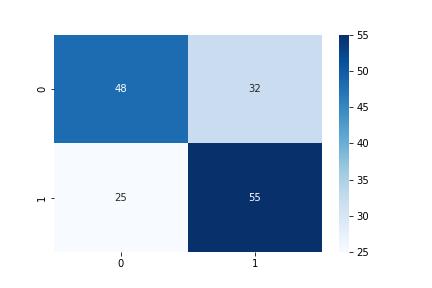
\includegraphics[width=\textwidth]{figures/ClassificationTree.png}
        \caption{Classification Tree}\label{dt cm}
    \end{subfigure}
    \begin{subfigure}[t]{0.45\textwidth}
        \centering
        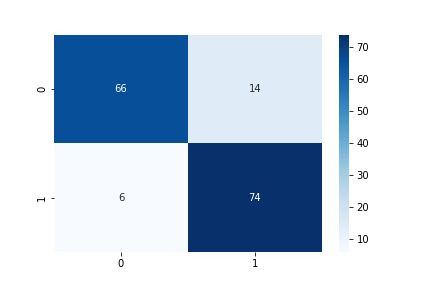
\includegraphics[width=\textwidth]{figures/RandomForest.png}
        \caption{Random Forest}\label{rf cm}
    \end{subfigure}
    \caption{Confusion Matrices}
\end{figure}

\begin{multicols}{2}

\section{Discussion}
In this section, we discuss the following five questions based on an analysis of the experimental procedure described above and the results obtained:
\begin{itemize}
    \item \emph{How does the performance of the generative linear model (multinomial naive Bayes) compare to the discriminative linear model (regularized logistic regression)? }
    \item \emph{Is the random forest able to improve on the performance of the linear classifiers? }
    \item \emph{Does performance improve by adding Bi-grams features, instead of using just Uni-grams?  }
    \item \emph{What are the five most important terms (features) pointing towards a fake review? }
    \item \emph{What are the five most important terms (features) pointing towards a genuine review?  }
\end{itemize}


\subsection{Logistic Regression and Multionmial Naive Bayes}
In order to compare the accuracy of comment classification under different models, we analyze and compare here the logistic regression model and the naive Bayes model, which we will describe and compare the performance of the generative linear model (multinomial naive Bayes) and the discriminative linear model (regularized logistic regression). The best F1 score for the multinomial naive Bayes classifier is about 0.8999 in some cases, while the best F1 score for logistic regression is about 0.8435.

In numerical terms, since the F1 score measures the accuracy of a binary classification model, it takes into account both the accuracy and recall of the classification model. Therefore, it is clear that multinomial naive Bayes has a much better classification performance than logistic regression. By comparing the other parameter values, we believe that the first reason is the difference between the two algorithms' models themselves. That is, multinomial naive Bayes is a generative model, whereas logistic regression is a discriminative model. 

The second reason is the conditional independence assumption of the multinomial naive Bayes method, which allows multinomial naive Bayes to use weights directly by counting the logistic occurrence ratio of each feature without using gradient descent. Also, from the elaboration of the model results in the previous section, for both models, we used the same ngrams, i.e., both Uni-grams and Bi-grams were used. In order to compare the degree of classification of the models, we trained each model using Uni-grams, Bi-grams, and both Uni-grams and Bi-grams separately. 

In the multinomial naive Bayes model, if we choose to use only Uni-grams, with stemming as FALSE, lemmatization as FALSE, and lowercase and remove stops as TRUE, the multinomial naive Bayes model has an F1 score of 0.8748, while logistic regression has an F1 score of 0.8309. Under the same premise, after converting the Uni-grams to Bi-grams, multinomial naive Bayes has an F1 score of 0.7360, while the F1 score for logistic regression becomes 0.6843. Again, under the same conditions, if we use both Uni-grams and Bi-grams, the F1 score for multinomial naive Bayes is 0.8935, while the F1 score for logistic regression is 0.8371. You can see a visualization of this in Figure \ref{results:n-grams}.

This result is very much in line with what would be expected when we use the same constraints. The model classification goes from worst to best using Bi-grams, to using Uni-grams, and the best case is using both Uni-grams and Bi-grams. This is because using both Uni-grams and Bi-grams allows for a greater degree of accurate text classification.

Furthermore, both models we obtained had high F1 scores due to our pre-processing of the text. If we set remove stop to FALSE, we are not removing all the stop words that occur often and do not have any meaning in the process of text mining. In this case, we obtain an F1 value of 0.8124 for multinomial naive Bayes, while the F1 value for logistic regression is greater than the value for multinomial naive Bayes, which is 0.8373. 

This occurs because multinomial naive Bayes focuses on using the probability of features for classification, and because we did not pre-process the text in advance, the features in the text are not obvious and there are many meaningless interference terms, which will cause the accuracy of multinomial naive Bayes model to decrease; while the constraints of logistic regression are lower compared to multinomial naive Bayes, and can use optimization methods such as gradient descent to obtain coupling information between features.

In summary, we have made a basic comparison of the two models in terms of their F1 values and analysed the two models by using a comparison of the F1 values of the two models in the cases of Uni-grams, Bi-grams and using both simultaneously. Finally, the two models were compared using whether or not pre-processing was performed. From the F1 values obtained, the classification of the two models is in line with our expectations. You can see a comparative chart of the two models in Figure \ref{fancy}.

\end{multicols}
\begin{figure}[h]
    \centering
    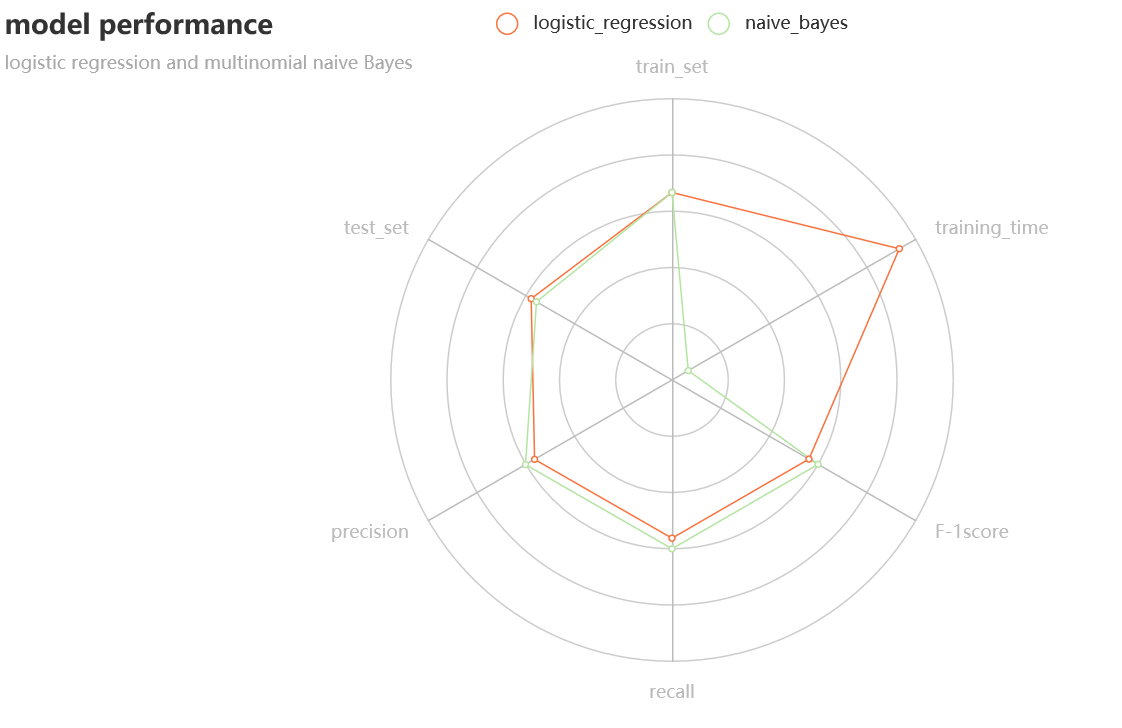
\includegraphics[width=0.545\textwidth]{figures/model_performance.png}
    \caption{Comparison of Logistic Regression and Naive Bayes.}\label{fancy}
\end{figure}
\begin{multicols}{2}


\subsection{N-grams}
From the comparison of F1 values described above, the random forest classifier improves the classifier's performance. Furthermore, for different classifiers, would text classification using Uni-grams be better than using Bi-grams for classification? Or perhaps using both Uni-grams and Bi-grams would give better classification results? In the previous section, we have made a basic comparison between the logistic regression classifier and the multinomial naive Bayes classifier using Uni-grams, Bi-grams, and both. The classification obtained using Bi-grams was worse than that obtained using Uni-grams, but the best classification results were obtained using both. 

The remaining two models, decision tree and random forest, are analyzed here. For the decision tree classifier model, when using only Uni-grams, and with pre-processing of no stemming or lematization, lowercased words, and removed stop words, the highest F1 is 0.644; In the same pre-processing case, but when using only Bi-grams, the highest F1 score was 0.600. However, with the words stemmed, lowercased and stop words removed, the decision tree classifier obtained an F1 score of 0.662 with Uni-grams, compared to 0.701 with Bi-grams. This is the best F1 score for the decision tree model, even higher than using both Uni-grams and Bi-grams. 

It seems that, for the first case, the use of Bi-grams did not improve the accuracy of the classifier. We believe that this is because we have the same tree. The drop in performance in our analysis is due to overfitting an overly large tree on the training data. However, if one were to use a more aggressive regularization strategy, such as one involving Minimal Cost-Complexity Pruning (chapter 3 of \cite{breiman2017classification}), the overfitting problem could be overcome. This may result in higher F1 scores when using Bi-grams than those obtained when using Uni-grams or both Uni-grams and Bi-grams.

For the random forest classifier model, the highest F1 score obtained with Uni-grams is 0.868, while the score obtained with Bi-grams is 0.774, and the score obtained with both Uni-grams and Bi-grams is 0.828. Therefore, the use of Bi-grams does not improve the performance of the classifier. Again, we believe that Bi-grams (or even n-gram) has a data sparsity problem. This may make them less informative.

As elaborated in the previous subsection, in logistic regression and multinomial naive Bayes, using Bi-grams does not improve the F1 score of this classifier model but instead decreases the model's performance, but using both Uni-grams and Bi-grams can improve the performance of the model. We assume that this is because it will have a smoothing effect.

In summary, random forest improves the performance of linear classifiers. However, using Bi-grams instead of Uni-grams does not improve the classifier's performance in random forest and decision trees. The same applies to logistic regression and multinomial naive Bayes, but unlike the first two classifiers, these two classifiers can rely on using both Uni-grams and Bi-grams to improve classifier performance.

\subsection{Most Important Features}

In table \ref{most important}, you can see the five most important words with deceptive features obtained by using the best performing classifier, Logistic Regression, are "\emph{chicage, smell, seem, luxuri, make}". The five most important feature terms pointing to true reviews are "\emph{great, locat, call, elev. star}". 

In the list of deceptive features, we can see that the negative value of \emph{chicago} is very large. Here, we use the magnitude of the value to indicate how trustworthy this feature value is. The smaller the value, the more likely the keyword is to be deceptive, while the larger the value, the more trustworthy and true the word is. 

From the above subsections, we have noted that we utilized Uni-gram, Bi-gram, and both Uni-gram and Bi-gram, but from the results, all the eigenvalues with larger values belong to Uni-gram. This is because adding Bi-gram to the classifier does not improve text classification performance, as we have already analyzed in the previous section. Furthermore, since the texts are all stemmed, we need to emphasize that some of the words collected here are not really words, since they have stems. For example, in the deceptive trait terminology, \emph{luxuri} is stemmed from both luxury and luxurious.

\end{multicols}
\begin{table}[h]
\centering
\caption{The 10 most informative features.}
\begin{tabular}{ll|ll}
\hline
\multicolumn{2}{l|}{\textbf{Deceptful}} & \multicolumn{2}{l}{\textbf{Truthful}} \\ \hline
N-gram             & Change             & N-gram            & Change            \\
chicago            & -0.6562            & great             & 0.3509            \\
smell              & -0.3865            & locat             & 0.3369            \\
seem               & -0.3176            & call              & 0.3206            \\
luxuri             & -0.3087            & elev              & 0.3161            \\
make               & -0.3050            & star              & 0.2766            \\ \hline
\end{tabular}
\label{most important}
\end{table}
\begin{multicols}{2}


\section{Conclusion and Future Work} % ;)
In this paper, we have analyzed the performance of the four models in detail and analyzed the results. However, when analyzing the performance of the parameters, we found that logistic regression and multinomial naive Bayes can be used to improve the classifier's performance using both Uni-gram and Bi-gram, but not decision tree and random forest. This was brought to our attention. Furthermore, it was noted that the different preprocessing conditions resulted in higher F1 scores for decision trees with Bi-gram than with Uni-gram. Why does it appear that the modification of the preprocessing only under the decision tree model leads to better results for the Bi-gram than the Uni-gram classification case? This is a question that could be explored in further research. Moreover, we considered using some of the other hyper-parameters available in scikit\-learn, such as ccp\_alpha to better train and correct the results.


\bibliographystyle{ieeetr}
\bibliography{mybib.bib}
\end{multicols}

\appendix

\section{Appendix}
\subsection{List of stop words, taken from the English list in NLTK}
\label{appendix:words}
\begin{lstlisting}
stops = ["i", "me", "my", "myself", "we", "our", "ours", "ourselves", "you", "your", "yours", 
"yourself", "yourselves", "he", "him", "his", "himself", "she", "her", "hers", "herself", "it",
"its", "itself", "they", "them", "their","theirs", "themselves", "what", "which", "who",
"whom", "this", "that", "these", "those", "am", "is", "are", "was", "were", "be", "been", 
"being", "have", "has", "had", "having", "do", "does", "did", "doing", "a", "an", "the",
"and", "but", "if", "or", "because", "as", "until", "while", "of", "at", "by", "for",
"with", "about", "against", "between", "into", "through", "during", "before", 
"after", "above", "below", "to", "from", "up", "down", "in", "out", "on", "off", "over", 
"under", "again", "further", "then", "once", "here", "there", "when", "where", "why", "how",
"all", "any", "both", "each", "few", "more", "most", "other", "some", "such", "no", "nor", 
"not", "only", "own", "same", "so", "than", "too", "very", "s", "t", "can", "will", "just",
"don", "should", "now"]  # stop word list taken from NLTK
\end{lstlisting}

\begin{sidewaysfigure}[ht]
    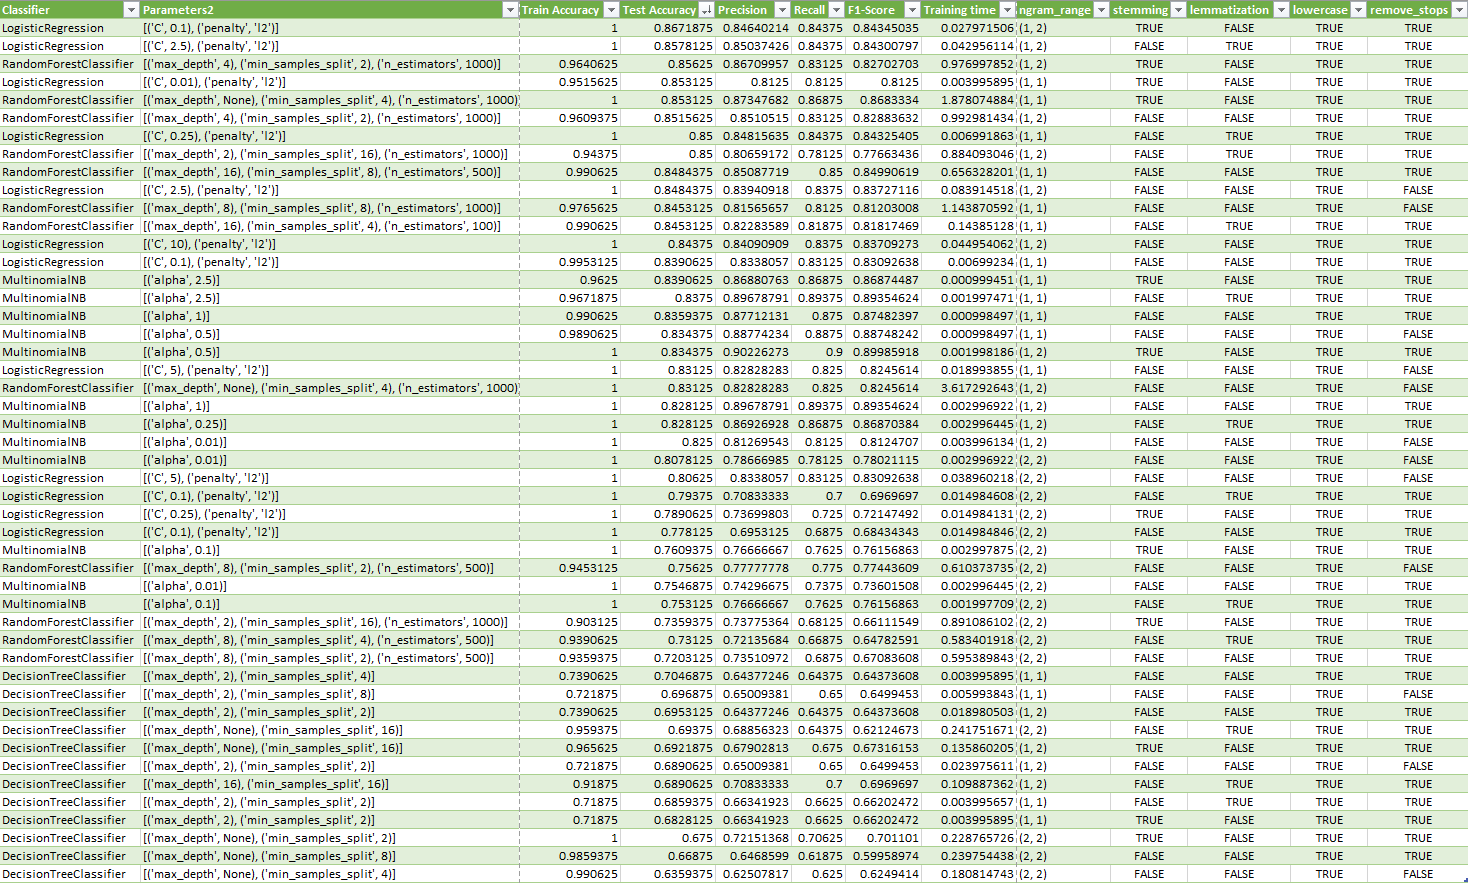
\includegraphics[width=\textwidth]{figures/Untitled.png}
    \caption{Table of results for best performing classifier in each pre-processing setting.}
    \label{apx:results}
\end{sidewaysfigure}
\onecolumn

\end{document}